% !TeX root = RJwrapper.tex
\title{MY Starwars Assignment}
\author{by James Lee}

\maketitle

\abstract{%
Abstract no abstract.
}

\hypertarget{introduction}{%
\subsection{Introduction}\label{introduction}}

Introductory section which may include references in parentheses
\citep{R}, or cite a reference such as \citet{R} in the text.

Let's try a citation here with \citet{barba2018terminologies} who says
useful things.

\hypertarget{section-title-in-sentence-case}{%
\subsection{Section title in sentence
case}\label{section-title-in-sentence-case}}

This section may contain a figure such as Figure \ref{fig:Rlogo}.

\begin{Schunk}
\begin{figure}[htbp]

{\centering 
\includegraphics[width=2in]{Rlogo} 

}

\caption[The logo of R]{The logo of R.}\label{fig:Rlogo}
\end{figure}
\end{Schunk}

\hypertarget{another-section}{%
\subsection{Another section}\label{another-section}}

There will likely be several sections, perhaps including code snippets,
such as:

\begin{Schunk}
\begin{Sinput}
print(df)
\end{Sinput}
\begin{Soutput}
#>                name height  mass  homeworld
#> 1    Luke Skywalker    172  77.0   Tatooine
#> 2    Obi-Wan Kenobi    182  77.0    Stewjon
#> 3  Anakin Skywalker    188  84.0   Tatooine
#> 4    Wilhuff Tarkin    180    NA     Eriadu
#> 5          Han Solo    180  80.0   Corellia
#> 6    Wedge Antilles    170  77.0   Corellia
#> 7  Jek Tono Porkins    180 110.0 Bestine IV
#> 8         Boba Fett    183  78.2     Kamino
#> 9        Mon Mothma    150    NA  Chandrila
#> 10     Arvel Crynyd     NA    NA       <NA>
#> 11     Qui-Gon Jinn    193  89.0       <NA>
#> 12    Finis Valorum    170    NA  Coruscant
#> 13   Shmi Skywalker    163    NA   Tatooine
#> 14      Cliegg Lars    183    NA   Tatooine
#> 15            Dooku    193  80.0    Serenno
#> 16       Jocasta Nu    167    NA  Coruscant
\end{Soutput}
\end{Schunk}

\begin{Schunk}
\begin{Sinput}
library(tidyverse)
library(dplyr)
library(plyr)
library(data.table)
data = starwars %>% filter(species == "Human")
df = data.table(data)
df %>% 
  ggplot(aes(x = height, 
             y = mass)) +
  geom_point()
\end{Sinput}
\begin{figure}
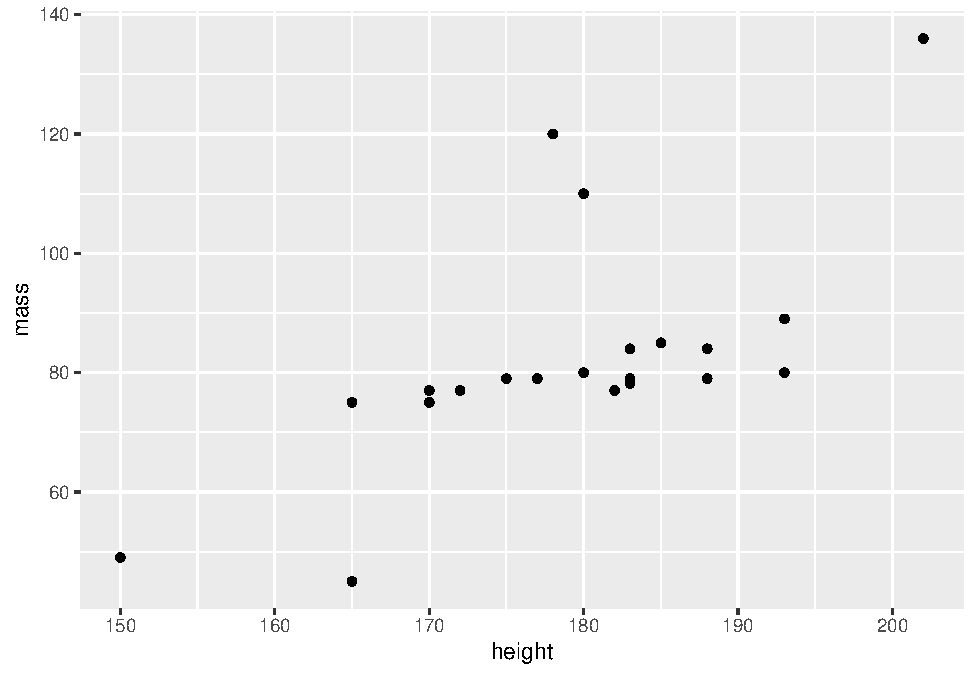
\includegraphics{Untitled_files/figure-latex/print-the-plot-1} \caption[a ggplot of stuf]{a ggplot of stuf}\label{fig:print-the-plot}
\end{figure}
\end{Schunk}

\hypertarget{summary}{%
\subsection{Summary}\label{summary}}

This file is only a basic article template. For full details of
\emph{The R Journal} style and information on how to prepare your
article for submission, see the
\href{https://journal.r-project.org/share/author-guide.pdf}{Instructions
for Authors}.

\bibliography{RJreferences}


\address{%
James Lee\\
University of Washington\\
line 1\\ line 2\\
}
\href{mailto:jlee0920@uw.edu}{\nolinkurl{jlee0920@uw.edu}}

